\section{Theorie}
\label{sec:Theorie}
\subsection{Das magnetische Moment und der Landéfaktor}
\label{sec:magmom}
Der Gesamtdrehimpuls einer Elektronenhülle kann mit dem magnetischen Moment beschrieben werden:
\begin{equation}
  \label{eqn:magneton}
  \vec{\mu}_\mathrm{J}=-g_\mathrm{J}\mu_\mathrm{B}\vec{J}
\end{equation}
Dabei ist $g_\mathrm{J}$ der Landéfaktor und $\mu_\mathrm{B}=\dfrac{e\hbar}{2m_\mathrm{e}}$ das bohrsche Magneton. Der Betrag ergibt sich zu:
\begin{equation}
  \label{absolute}
  |\vec{\mu}_\mathrm{J}|=g_\mathrm{J}\mu_\mathrm{B}\sqrt{J(J+1)}
\end{equation}
Desweiteren gelten für Bahndrehimpuls bzw. Spin die folgenden Zusammenhänge:
\begin{align}
  \vec{\mu}_\mathrm{L}&=-\mu_\mathrm{B}\vec{L} \\
  |\vec{\mu}_\mathrm{L}|&=\mu_\mathrm{B}\sqrt{L(L+1)} \\
  \vec{\mu}_\mathrm{S}&=-g_\mathrm{S}\mu_\mathrm{B}\vec{S} \\
  |\vec{\mu}_\mathrm{S}|&=g_\mathrm{S}\mu_\mathrm{B}\sqrt{S(S+1)}
\end{align}
Dabei ist $g_\mathrm{S}$ der Landé-Faktor des freien Elektrons. Dieser ist mit $g_\mathrm{S}=2.00232$ gegeben.
Der Landé-Faktor $g_\mathrm{J}$ beschreibt die Zusammensetzung des Gesamtdrehimpulses aus Bahndrehimpuls und Spin. Es wirkt nur noch $\vec{\mu}_\mathrm{J}$ als magnetisches Moment, da durch die Präzessionsbeweg um $\vec{J}$ nur die parallelen Komponenten $\vec{\mu}_\mathrm{J}$ verbleiben. Damit folgt für den Landé-Faktor $g_\mathrm{J}$:
\begin{equation}
  \label{eqn:lande}
  g_\mathrm{J}=\dfrac{3.0023J(J+1)+1.0023[S(S+1)-L(L+1)]}{2J(J+1)}
\end{equation}
Durch den Zeemann-Effekt werden bei angelegtem Magnetfeld $\vec{B}$ die Energieniveaus in $2J+1$ Unterniveaus aufgespalten. Durch die Richtungsquantelung $U_\mathrm{mag}=-\vec{\mu}_\mathrm{J}\cdot\vec{B}$ folgt, dass $U_\mathrm{mag}$
nur ganzzahlige Vielfache von $g_\mathrm{J}\mu_\mathrm{B}B$ annehmen kann also:
\begin{equation}
  \label{eqn:mj}
  U_\mathrm{mag}=M_\mathrm{J}g_\mathrm{J}\mu_\mathrm{B}B
\end{equation}
Dabei ist $M_\mathrm{J}\in[-J,...,J]$.
\subsection{Hyperfeinstruktur}
Für das betrachtete Rubidium ist der Kernspin $\vec{I}\neq 0$. Dadurch bildet sich die sogenannte Hyperfeinstruktur.
Durch die Kopplung des Bahndrehimpulses der Elektronenhülle $\vec{J}$ an den Spin des Kerns $\vec{I}$ verändert sich damit die Zeemannaufspaltung. Es ergibt sich der Gesamtdrehimpuls $\vec{F}$:
\begin{equation}
  \label{eqn:gesamtdre}
  \vec{F}=\vec{J}+\vec{I}
\end{equation}
Durch die Beeinflussung des magnetischen Momentes des Kerns durch das von der Elektronenhülle induzierte B-Feld wird die neue Quantenzahl $F$ eingeführt. Dabei ist $F \in [|I-J|,...,|I+J|]$. $F$ gibt die Anzahl der Hyperfeinstrukturaufspaltungen an. In Abschnitt \ref{sec:magmom} wurde die Quantenzahl $M_\mathrm{J}$ eingeführt, diese wird nun durch $M_\mathrm{F}$ mit $M_\mathrm{F} \in [-F,...,F]$ ersetzt, damit wird Gleichung (\ref{eqn:mj}) für
die Energien der Aufspaltungen angepasst zu:
\begin{equation}
  \label{eqn:mf}
  U_\mathrm{HF}=M_\mathrm{F}g_\mathrm{F}\mu_\mathrm{B}B
\end{equation}
Der neu eingeführte Landé-Faktor $g_\mathrm{F}$ kann wie folgt angegeben werden:
\begin{equation}
  \label{eqn:gf}
  g_\mathrm{F}\approx g_\mathrm{J}\dfrac{F(F+1)+J(J+1)-I(I+1)}{2F(F+1)}
\end{equation}
\subsection{Optisches Pumpen}
\label{sec:op}
Es werden zwei Zustände auf der Atomschale betrachtet mit den jeweiligen Energien $E_\mathrm{1}$ und $E_\mathrm{2}$ für die gilt $E_\mathrm{2}>E_\mathrm{1}$. Die Besetzung der Zustände im thermischen Gleichgewicht ist gegeben durch:
\begin{equation}
  \label{eqn:oppu}
  \dfrac{N_\mathrm{2}}{N_\mathrm{1}}=\dfrac{g_\mathrm{2}}{g_\mathrm{1}}\exp(-\dfrac{E_\mathrm{2}-E_\mathrm{1}}{k_\mathrm{b}T})
\end{equation}
Nun lässt sich mit der Methode des optischen Pumpen eine Inversion der Energieverteilung nach Gleichung (\ref{eqn:oppu}) erzeugen. Um diese Inversion aufrecht zu erhalten muss dem betrachteten Sytem ständig Energie zugeführt werden, dies geschieht durch das optische Pumpen. Bei der Invesion werden nun nur noch Photonen der Energie $h\nu=E_\mathrm{2}-E_\mathrm{1}$ erzeugt.
In Abbildung (\ref{fig:niveaus}) sind die Übergänge für ein Alkali-Atom dargestellt:
\begin{figure}[h!]
  \centering
  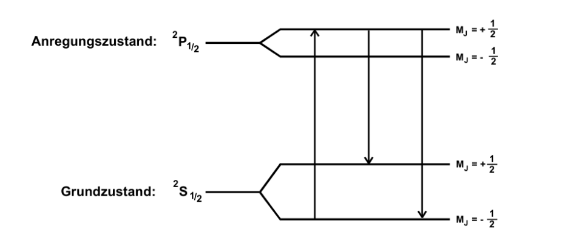
\includegraphics[scale=0.5]{fig/niveaus.png}
  \caption{Aufspaltung eines Alkaliatoms mit den dazugehörigen Übergängen.}
  \label{fig:niveaus}
\end{figure}
Polarisierte Licht sorgt für ein Übergang eines Elektrons zum Zustand $\Delta M=\pm 1$. Rechtszirkular-polarisiertes Licht sorgt dabei für $\Delta M=+1$, linkszirkular-polarisiertes Licht für $\Delta M=-1$.
Bei der Nutzung nur rechtszirkular-polarisiertes Licht, wird nur der niedrige Zustand $S_\mathrm{1/2}$ mit $M=-\dfrac{1}{2}$ angeregt, da der höhere Zustand $S_\mathrm{1/2}$ mit $M=\dfrac{1}{2}$ keinen angeregten Zustand besitzt,
der die Auswahlregeln  $\Delta M=+1$, erfüllt. Die Elektronen im angeregten Zustand $P_\mathrm{1/2}$ mit $M=\dfrac{1}{2}$ gehen durch spontane Emissionen mit gleicher Wahrscheinlichkeit in die beiden Grundzustände über. Dadurch wird das untere Energieniveau leer „gepumpt“ und es entsteht eine Besetzungszahlinversion zu $S_\mathrm{1/2}$ mit $M=\dfrac{1}{2}$. Dies ist in Abbildung (\ref{fig:12}) dargestellt:
\begin{figure}[h!]
  \centering
  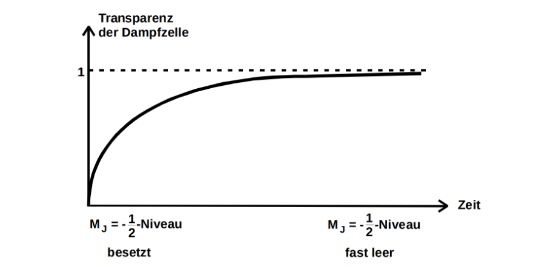
\includegraphics[scale=0.7]{fig/12.png}
  \caption{Transparenz der Apparatur aufgetragen gegen die Zeit.}
  \label{fig:12}
\end{figure}
\subsection{Hochfrequenzspektronomie}
\label{sec:hfsp}
Das Verfahren des Optischen Pumpen kann zur Messung des Abstandes zweier Energieniveaus genutzt werden. Es gibt zwei Möglichkeiten, die nach einer Besetzungszahlinversion eintreten können: die spontane Emission und die induzierte Emission. Dabei wird im Hochfrequenzfeld ein Photon erzeugt. Das Elektron geht dann in den Grundzustand über, indem es ein Photon mit gleicher Frequenz, Polarisation und Energie emittiert. Das Photon benötigt dafür die Energie aus Gleichung (\ref{eqn:mf}). \\
Welche der beiden Emissionsarten überwiegt ist frequenzabhängig. Im Bereich der Zeemann-Aufspaltung kann die spontane Emission vernachlässigt werden. Dadurch, dass das Erdmagnetfeld als Nullfeld wirkt ist das optische Pumpen jedoch unmöglich. Zu dessen Kompensation wird ein einstellbares Hochfrequenzfeld angelegt und damit das Erdmagnetfeld gemessen um dieses als Störfaktor zu entfernen. Damit lässt sich nun die Inversion aus Abschnitt (\ref{sec:op}) herbeiführen.
Dafür wird die Transparenz der Apparatur maximal. Erhöht man das Magnetfeld lässt sich die induzierte Emission auslösen. Dies passiert genau dann wenn gilt:
\begin{equation}
  \label{eqn:bm}
  h\nu=\Delta M_\mathrm{J}g_\mathrm{J}\mu_\mathrm{B}B_\mathrm{m}
\end{equation}
In Abbildung (\ref{fig:transpa}) ist dies schematisch dargestellt:
\begin{figure}[h!]
  \centering
  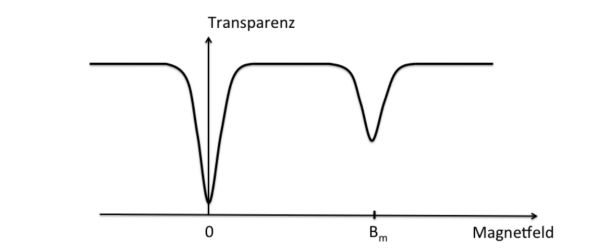
\includegraphics[scale=0.5]{fig/transpa.png}
  \caption{Transparenz der Apparatur aufgetragen gegen das Magnetfeld.}
  \label{fig:transpa}
\end{figure}
\subsection{Quadratischer Zeeman-Effekt}
\label{sec:quadr}
Wird das Magnetfeld größer müssen für die Übergangsenergie auch Terme höherer Ordnung berücksichtigt werden, die Energie aus Gleichung (\ref{eqn:mf}) wird dann zu:
\begin{equation}
  \label{eqn:quadra}
  U_\mathrm{HF}=g_\mathrm{F}\mu_\mathrm{B}B+g_\mathrm{F}^2\mu_\mathrm{B}^2B^2\dfrac{1-2M_\mathrm{F}}{\Delta E_\mathrm{HF}}
\end{equation}
Dabei ist $\Delta E_\mathrm{HF}$ die Energiedifferenz der Hyperfeinstruktur der Niveaus $F$ und $F+1$
